\classheader{2018-09-12}
\subsection*{Half spaces, Hyperplanes, Polyhedral sets}
\textbf{Recall: } Suppose $p,x \in \mathbb{R}^n$. The inner product of $p,x$
\begin{gather*}
	p^Tx = \left||p|\right| \left||x|\right| \cos \theta\\
	\text{thus } p^Tx 
	\begin{cases}
		> 0 & \text{if $\theta$ acute}\\
		= 0 & \text{if $p \perp x$ (perpendicular)}\\
		< 0 & \text{if $\theta$ obtuse}\\
	\end{cases}
\end{gather*}
\begin{definition-N}
	Suppose $p \in \mathbb{R}^n$ non-zero. $\{\vec{x} \in \mathbb{R}^n : p^T x = 0 \}$ is a hyperplane through origin with normal vector $p$. $\{\vec{x} \in \mathbb{R}^n : p^T x \leq 0 \}$ is (associated) and (closed) half space.
\end{definition-N}
\textbf{Example}
	\begin{center}
		\begin{tikzpicture}
		\coordinate (A) at (0,-1);
  		\coordinate (B) at (0,4);
  		\coordinate (C) at (4,0);
  		\coordinate (D) at (-4,0);
		\coordinate (E) at (2,3);
		\coordinate (F) at (0,0);
		\coordinate (G) at (-3,2);
		\coordinate (H) at (3,-2);
  		%\draw [->] (A) -- (B) node [pos=.9, auto, swap] {$b_1$} node [pos=.9, auto] {$C$} ;
  		%\draw [->] (A) -- (C) node [pos=.9, auto] {$b_2$} ;
  		\draw[->, line width=0.5mm] (F) -- (E) node [pos = .9, auto, swap] {$\vec{p} = \begin{bmatrix}
  			2\\3
  		\end{bmatrix}$};
  		\draw [<->] (C) -- (D) node[pos = .9, auto, swap] {$x$};
  		\draw [<->] (A) -- (B) node[pos = .9, auto, swap] {$y$};
  		\draw [densely dotted] (G) -- (H) node[pos = .9, auto] {perp to p $\rightarrow$ hyperplane};
	\end{tikzpicture}
	\end{center}
Everything on either side of the hyperplane is the \emph{half spaces}.
\begin{definition-N}
	In general \emph{hyperplanes} in $\mathbb{R}^n$ are sets $\{x \in \mathbb{R}^n, p^Tx = \alpha \}$ for non-zero $p \in \mathbb{R}^n$, and $\alpha \in \mathbb{R}$
\end{definition-N}
\begin{definition-N}
	\emph{half spaces} in $\mathbb{R}^n$ are sets $\{x \in \mathbb{R}^n, p^Tx \geq \alpha \}$ for non-zero $p \in \mathbb{R}^n$, and $\alpha \in \mathbb{R}$
\end{definition-N}
\begin{example-N}
	\begin{align*}
		\text{(2D)} \hspace{4.8em} 2x_1 + 5x_2 = 6 \qquad & \text{hyperplane}\\
		2x_1 + 5x_2 \geq 6 \qquad & \text{half space}\\
		\text{(3D)} \qquad 3x_1 + 2x_2 - 7x_3 = 8 \qquad & \text{hyperplane}\\
		3x_1 + 2x_2 - 7x_3 \geq 8 \qquad & \text{half space}
	\end{align*}
\end{example-N}
\begin{definition-N}
	A \emph{polyhedron} (polyhedral space) is the intersection of finely may half spaces.
	\begin{example-N}
		$x \cdot Ax \geq b$ for $A \in \mathbb{R}^{mxn}, \quad b \in \mathbb{B}^m$
		\begin{gather*}
			\begin{matrix}
				\vec{p_1} \rightarrow\\
				\vec{p_2} \rightarrow\\
				\vdots\\
				\vec{p_m} \rightarrow
			\end{matrix}
			\begin{bmatrix}
				a_{11} & a_{12} & a_{13} & \ldots & a_{1n}\\
				a_{21} & a_{22} & a_{23} & \ldots & a_{2n}\\
				\vdots & \vdots & \ddots & \ddots & \vdots\\
				a_{m1} & a_{m2} & a_{m3} & \ldots & a_{mn}
			\end{bmatrix}
			\begin{bmatrix}
				x_1 \\ x_2\\ \vdots\\ x_n
			\end{bmatrix} \geq
			\begin{bmatrix}
				b_1\\ b_2\\ \vdots\\ b_m
			\end{bmatrix}
		\end{gather*}
		$\vec{x}$ satisfies $Ax \geq b$ \underline{iff} $\vec{x}$ satisfies ${p_1}^Tx \geq b_1$, and $\vec{x}$ satisfies ${p_2}^Tx \geq b_2$, $\ldots$, ${p_m}^Tx \geq b_m$
	\end{example-N}
\end{definition-N}
\begin{example-N}
	\begin{gather*}
		\begin{bmatrix}
			1 & -2\\
			-1 & -1\\
			1 & 0\\
			0 & 1
		\end{bmatrix}
		\begin{bmatrix}
			x_1\\ x_2
		\end{bmatrix} \geq
		\begin{bmatrix}
			-6 \\ -5 \\ 0\\0
		\end{bmatrix}
	\end{gather*}
	\begin{multicols}{2}
		\begin{enumerate}
			\item $x_1 - 2x_2 \geq -6$
			\item $-x_1 -x_2 \geq 5$
			\item $x_1 \geq 0$
			\item $x_2 \geq 0$
		\end{enumerate}	
		\end{multicols}
		\begin{center}
			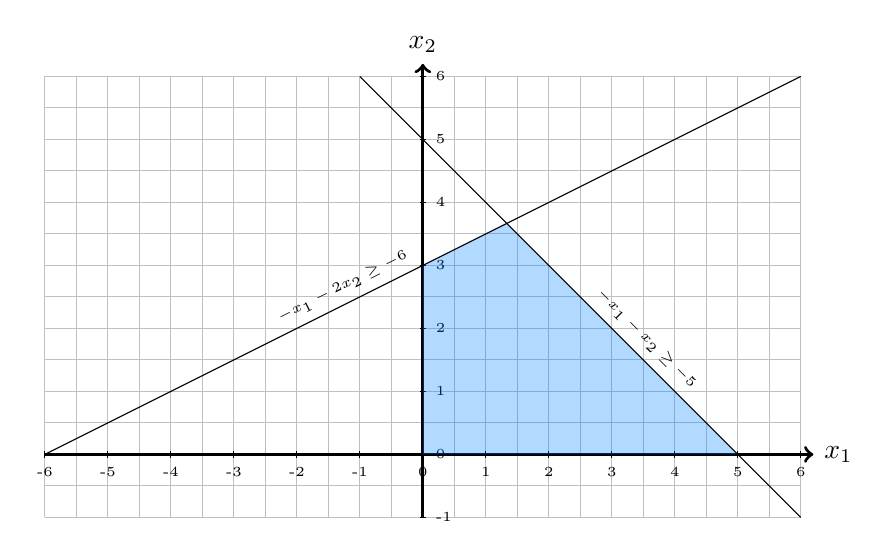
\begin{tikzpicture}[scale=0.8]

    		\draw[gray!50, thin, step=0.5] (-6,-1) grid (6,6);
    		\draw[very thick,->] (-6,0) -- (6.2,0) node[right] {$x_1$};
		    \draw[very thick,->] (0,-1) -- (0,6.2) node[above] {$x_2$};

		    \foreach \x in {-6,...,6} \draw (\x,0.05) -- (\x,-0.05) node[below] {\tiny\x};
		    \foreach \y in {-1,...,6} \draw (-0.05,\y) -- (0.05,\y) node[right] {\tiny\y};

		    \fill[blue!50!cyan,opacity=0.3] (0,0) -- (0,3) -- (4/3,11/3) -- (5,0)--  cycle;

		    \draw (-6,0) -- node[above left,sloped] {\tiny$-x_1-2x_2\geq-6$} (6,6);
		    \draw (-1,6) -- node[above right,sloped] {\tiny$-x_1-x_2\geq-5$} (6,-1);
			\end{tikzpicture}
		\end{center}
		\textbf{Solving (LP) geometrically}\\
		\begin{gather*}
			\begin{split}
				\text{min} \qquad & \begin{bmatrix}
					1\\-3
				\end{bmatrix}^T \begin{bmatrix}
					x_1\\x_2
				\end{bmatrix}\\
				\text{s.t.} \qquad & \begin{bmatrix}
					1 & -2\\
					-1 & -1
				\end{bmatrix} \geq 
				\begin{bmatrix}
					-6\\-5
				\end{bmatrix}\\
				& x_1 \geq 0, x_2 \geq 0
			\end{split}\hspace{4em}
			\begin{split}
				\textbf{polyhedral sets:}\\
				x: Ax \leq b \equiv \quad & [(-A)x \geq (-b)]\\
				x: Ax = b \equiv \quad & \begin{bmatrix}
					Ax \geq b\\
					Ax \leq b
				\end{bmatrix} \quad \text{i.e.} \begin{bmatrix}
					A\\-A
				\end{bmatrix} x \geq \begin{bmatrix}
					b\\-b
				\end{bmatrix}\\
				x: \underbrace{Ax = b}_{x \geq 0} \equiv \quad & \begin{bmatrix}
					A\\-A\\I
				\end{bmatrix} x \geq \begin{bmatrix}
					b\\-b\\ \vec{0}
				\end{bmatrix}
			\end{split}
		\end{gather*}
		\begin{definition}
			\underline{$\alpha$-level set} is $\{x: f(x) = \alpha \}$	
		\end{definition}
		Here $\alpha$-level set is $x: x_1 - 3x_2 = \alpha$ \qquad rewrite: $x_2 = \underbrace{\frac{1}{3}}_{\text{slope}} x - \underbrace{\frac{\alpha}{3}}_{\text{y-int}}$	\\
		\begin{multicols}{2}
		\begin{center}	
		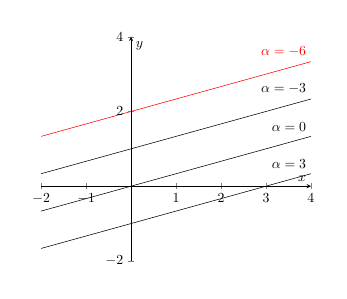
\begin{tikzpicture}[scale=0.5]
			\begin{axis}[
			xmin =-2, xmax=4,
			ymin=-2, ymax =4,
			axis lines=center,
			axis on top=true,
			domain=-2:4,
			xlabel={$x$},
    		ylabel={$y$},]
						
			\addplot[mark=none, draw=black, thin]{x/3 - 3/3} node [above left, pos=1] {$\alpha = 3$};
			\addplot[mark=none, draw=black, thin]{x/3 - 0/3} node [above left, pos=1] {$\alpha = 0$};
			\addplot[mark=none, draw=black, thin]{x/3 + 3/3} node [above left, pos=1] {$\alpha = -3$};
			\addplot[mark=none, draw=black, thin, red]{x/3 + 6/3} node [above left, pos=1] {$\alpha = -6$};
			\end{axis}
		
		\end{tikzpicture}
		\end{center}
			The solution is the level set with the least $\alpha$. In this case, $\alpha = -6$
		\end{multicols}
\end{example-N}